
	% Table 1: Experimental setup
	% ---------------------------------------------------------------
	\begin{table}[htbp]
		\centering
		\caption{Esquema del experimento para 10-fold cross-validation.}
		\label{tab:setup}
		\begin{tabular}{@{}ll@{}}
			\toprule
			Parametros & Valor \\
			\midrule
			Tamaño de la matriz & $610 \times 9724$ \\
			Valores observados & 100\,836 (1.70\% dense) \\
			Número de folds & 10 \\
			Factores elegidos $k$ & 2, 5, 8, 10, 20, 30, 50 \\
			$\lambda$ & 0.01 \\
			$\gamma$ & 0.01 \\
			Iteraciones maximas& 1000 \\
			Tolerancia & $10^{-4}$ \\
			\bottomrule
		\end{tabular}
	\end{table}
	
	% ---------------------------------------------------------------
	% Table 2: Summary of all combinations (ranked by mean test RMSE)
	% ---------------------------------------------------------------
	\begin{table}[htbp]
		\centering
		\caption{Resultados de la validación cruzada, listados por RMSE.
			The generalization gap is the mean test RMSE minus the mean train RMSE.}
		\label{tab:summary}
		\begin{tabular}{@{}rrrrrrrrr@{}}
			\toprule
			$k$ & $\lambda$ & Test RMSE & SD & Train RMSE & SD& Iteraciones & Convergencia & Tiempo \\
			\midrule
			2 & 0.01 & 1.0893 & 0.0100 & 0.7463 & 0.3431 &  47 & 10/10 & 6m 33.1s  \\
			5 & 0.01 & 1.1060 & 0.0129 & 0.6393 & 0.4667 &  60 & 10/10 & 8m 24.1s  \\
			8 & 0.01 & 1.1367 & 0.0125 & 0.5680 & 0.5688 &  67 & 10/10 & 9m 50.7s  \\
			10 & 0.01 & 1.1451 & 0.0123 & 0.5278 & 0.6173 &  68 & 10/10 & 9m 52.3s  \\
			50 & 0.01 & 1.1891 & 0.0117 & 0.1545 & 1.0346 & 108 & 10/10 & 16m 51.4s \\
			20 & 0.01 & 1.1907 & 0.0182 & 0.3726 & 0.8181 &  85 & 10/10 & 12m 21.3s \\
			30 & 0.01 & 1.1999 & 0.0096 & 0.2748 & 0.9250 &  90 & 10/10 & 13m 39.5s \\
			\bottomrule
		\end{tabular}
	\end{table}
	
	% ---------------------------------------------------------------
	% Table 3: Per-fold test RMSE
	% ---------------------------------------------------------------
	\begin{table}[h]
		\centering
		\caption{Test RMSE per fold for each number of factors $k$ ($\lambda = 0.01$).}
		\label{tab:fold-test}
		\begin{tabular}{@{}lrrrrrrr@{}}
			\toprule
			& \multicolumn{7}{c}{Number of factors $k$} \\
			\cmidrule(l){2-8}
			Fold & 2 & 5 & 8 & 10 & 20 & 30 & 50 \\
			\midrule
			1  & 1.1014 & 1.1204 & 1.1484 & 1.1624 & 1.2143 & 1.2176 & 1.2005 \\
			2  & 1.0882 & 1.1042 & 1.1412 & 1.1379 & 1.1826 & 1.2004 & 1.1906 \\
			3  & 1.1006 & 1.1238 & 1.1562 & 1.1561 & 1.2061 & 1.2070 & 1.2019 \\
			4  & 1.0831 & 1.1003 & 1.1283 & 1.1314 & 1.1743 & 1.1944 & 1.1856 \\
			5  & 1.1018 & 1.1163 & 1.1509 & 1.1655 & 1.2169 & 1.2050 & 1.2103 \\
			6  & 1.0729 & 1.0895 & 1.1178 & 1.1323 & 1.1624 & 1.1890 & 1.1728 \\
			7  & 1.0861 & 1.0957 & 1.1303 & 1.1350 & 1.1798 & 1.1994 & 1.1869 \\
			8  & 1.0794 & 1.0869 & 1.1311 & 1.1420 & 1.1775 & 1.1981 & 1.1820 \\
			9  & 1.0849 & 1.1081 & 1.1244 & 1.1447 & 1.1989 & 1.1836 & 1.1783 \\
			10 & 1.0948 & 1.1148 & 1.1387 & 1.1435 & 1.1939 & 1.2037 & 1.1825 \\
			\midrule
			Mean & 1.0893 & 1.1060 & 1.1367 & 1.1451 & 1.1907 & 1.1999 & 1.1891 \\
			SD   & 0.0100 & 0.0129 & 0.0125 & 0.0123 & 0.0182 & 0.0096 & 0.0117 \\
			\bottomrule
		\end{tabular}
	\end{table}
	
	% ---------------------------------------------------------------
	% Table 4: Per-fold final train RMSE
	% ---------------------------------------------------------------
	\begin{table}[htbp]
		\centering
		\caption{Final train RMSE per fold for each number of factors $k$ ($\lambda = 0.01$).
			The initial train RMSE was approximately 3.653 in every fold.}
		\label{tab:fold-train}
		\begin{tabular}{@{}lrrrrrrr@{}}
			\toprule
			& \multicolumn{7}{c}{Number of factors $k$} \\
			\cmidrule(l){2-8}
			Fold & 2 & 5 & 8 & 10 & 20 & 30 & 50 \\
			\midrule
			1  & 0.7418 & 0.6375 & 0.5636 & 0.5297 & 0.3588 & 0.2688 & 0.1475 \\
			2  & 0.7538 & 0.6376 & 0.5646 & 0.5280 & 0.3752 & 0.2739 & 0.1485 \\
			3  & 0.7485 & 0.6336 & 0.5645 & 0.5216 & 0.3694 & 0.2746 & 0.1531 \\
			4  & 0.7399 & 0.6412 & 0.5660 & 0.5325 & 0.3829 & 0.2801 & 0.1484 \\
			5  & 0.7416 & 0.6362 & 0.5621 & 0.5228 & 0.3607 & 0.2771 & 0.1529 \\
			6  & 0.7532 & 0.6369 & 0.5747 & 0.5325 & 0.3808 & 0.2686 & 0.1603 \\
			7  & 0.7525 & 0.6464 & 0.5717 & 0.5269 & 0.3876 & 0.2818 & 0.1571 \\
			8  & 0.7409 & 0.6595 & 0.5680 & 0.5211 & 0.3741 & 0.2702 & 0.1570 \\
			9  & 0.7560 & 0.6316 & 0.5742 & 0.5284 & 0.3643 & 0.2928 & 0.1464 \\
			10 & 0.7344 & 0.6325 & 0.5699 & 0.5340 & 0.3720 & 0.2601 & 0.1742 \\
			\midrule
			Mean & 0.7463 & 0.6393 & 0.5680 & 0.5278 & 0.3726 & 0.2748 & 0.1545 \\
			\bottomrule
		\end{tabular}
	\end{table}
	
	% ---------------------------------------------------------------
	% Table 5: Per-fold epochs to convergence
	% ---------------------------------------------------------------
	\begin{table}[htbp]
		\centering
		\caption{Epochs until convergence per fold for each number of factors $k$
			($\lambda = 0.01$). All 70 fits converged.}
		\label{tab:fold-epochs}
		\begin{tabular}{@{}lrrrrrrr@{}}
			\toprule
			& \multicolumn{7}{c}{Number of factors $k$} \\
			\cmidrule(l){2-8}
			Fold & 2 & 5 & 8 & 10 & 20 & 30 & 50 \\
			\midrule
			1  &  55 &  60 & 75 & 65 & 111 &  99 & 124 \\
			2  &  36 &  60 & 72 & 71 &  81 &  89 & 119 \\
			3  &  41 &  70 & 69 & 75 &  85 &  90 & 107 \\
			4  &  49 &  53 & 68 & 60 &  70 &  81 & 121 \\
			5  &  55 &  61 & 74 & 71 & 103 &  85 & 109 \\
			6  &  37 &  64 & 60 & 63 &  75 & 100 &  97 \\
			7  &  36 &  48 & 62 & 67 &  65 &  81 & 101 \\
			8  &  55 &  38 & 69 & 80 &  81 &  94 & 102 \\
			9  &  35 &  73 & 59 & 69 &  98 &  70 & 125 \\
			10 &  67 &  72 & 66 & 64 &  84 & 113 &  80 \\
			\midrule
			Mean & 47 & 60 & 67 & 68 & 85 & 90 & 108 \\
			Min  & 35 & 38 & 59 & 60 & 65 & 70 &  80 \\
			Max  & 67 & 73 & 75 & 80 & 111 & 113 & 125 \\
			\bottomrule
		\end{tabular}
	\end{table}
	
	% ---------------------------------------------------------------
	% Table 6: Per-fold running time (seconds)
	% ---------------------------------------------------------------
	\begin{table}[htbp]
		\centering
		\caption{Running time per fold in seconds for each number of factors $k$
			($\lambda = 0.01$). The last row gives the total time per combination.}
		\label{tab:fold-time}
		\begin{tabular}{@{}lrrrrrrr@{}}
			\toprule
			& \multicolumn{7}{c}{Number of factors $k$} \\
			\cmidrule(l){2-8}
			Fold & 2 & 5 & 8 & 10 & 20 & 30 & 50 \\
			\midrule
			1  & 45.6 & 50.2 & 61.9 & 54.4 &  99.2 &  92.2 & 123.0 \\
			2  & 29.3 & 50.2 & 63.6 & 63.6 &  72.1 &  81.1 & 111.6 \\
			3  & 38.0 & 58.5 & 65.4 & 65.2 &  71.2 &  81.5 & 100.5 \\
			4  & 41.4 & 44.2 & 62.3 & 50.4 &  58.1 &  73.7 & 113.6 \\
			5  & 46.5 & 50.4 & 63.2 & 59.7 &  87.0 &  76.7 & 100.1 \\
			6  & 30.9 & 53.4 & 54.6 & 53.8 &  62.2 &  90.6 &  87.3 \\
			7  & 30.0 & 40.6 & 53.5 & 61.8 &  55.1 &  73.1 &  88.0 \\
			8  & 46.5 & 31.9 & 59.2 & 69.4 &  71.9 &  84.6 &  97.3 \\
			9  & 29.0 & 63.6 & 50.8 & 59.0 &  85.9 &  63.7 & 115.4 \\
			10 & 55.8 & 61.0 & 55.9 & 54.8 &  78.6 & 102.1 &  74.4 \\
			\midrule
			Total & 6m 33.1s & 8m 24.1s & 9m 50.7s & 9m 52.3s & 12m 21.3s & 13m 39.5s & 16m 51.4s \\
			\bottomrule
		\end{tabular}
	\end{table}
	
	% ---------------------------------------------------------------
	% Table 7: Final refit on all data (k = 2, lambda = 0.01)
	% ---------------------------------------------------------------
	\begin{table}[htbp]
		\centering
		\caption{SGD refit on all 100\,836 observed ratings with the best combination
			($k = 2$, $\lambda = 0.01$, $\gamma = 0.01$). Total drop in RMSE: 2.9080 (79.6\%);
			run time 52.7\,s.}
		\label{tab:refit}
		\begin{tabular}{@{}rrr@{}}
			\toprule
			Iteration & Train RMSE & Change in RMSE \\
			\midrule
			0 (init)        & 3.6535 & --       \\
			10              & 0.8364 & 0.014911 \\
			20              & 0.7779 & 0.003289 \\
			30              & 0.7613 & 0.000408 \\
			40              & 0.7530 & 0.000555 \\
			50              & 0.7480 & 0.000394 \\
			55 (converged)  & 0.7455 & 0.000073 \\
			\bottomrule
		\end{tabular}
	\end{table}

	\begin{figure}[ht]
		\centering
		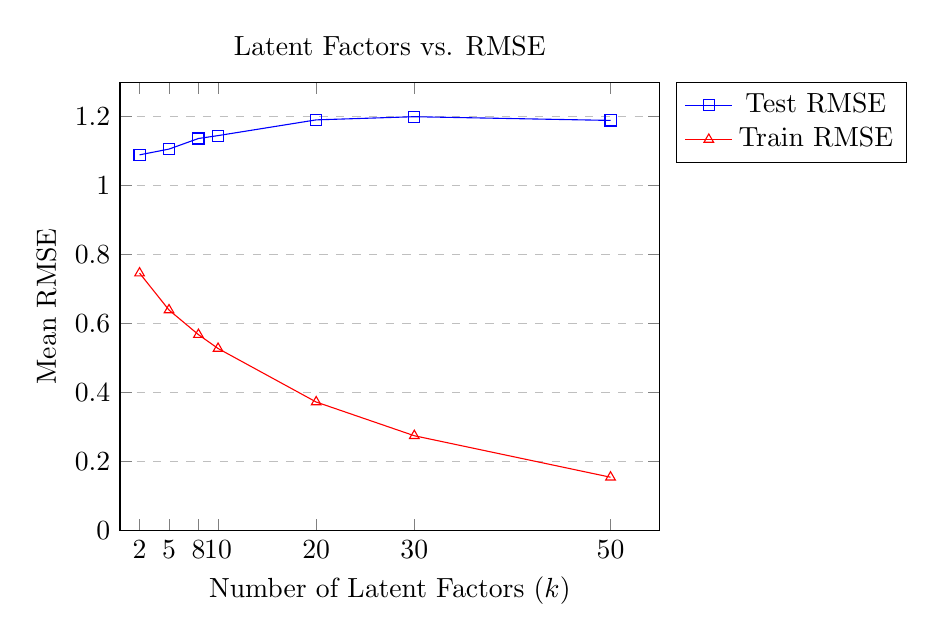
\begin{tikzpicture}
			\begin{axis}[
				title={Latent Factors vs. RMSE},
				xlabel={Number of Latent Factors (\(k\))},
				ylabel={Mean RMSE},
				xmin=0, xmax=55,
				ymin=0, ymax=1.3,
				xtick={2, 5, 8, 10, 20, 30, 50},
				legend pos=outer north east,
				ymajorgrids=true,
				grid style=dashed,
				]
				
				% Test RMSE
				\addplot[
				color=blue,
				mark=square,
				]
				coordinates {
					(2,1.0893)(5,1.1060)(8,1.1367)(10,1.1451)(20,1.1907)(30,1.1999)(50,1.1891)
				};
				\addlegendentry{Test RMSE}
				
				% Train RMSE
				\addplot[
				color=red,
				mark=triangle,
				]
				coordinates {
					(2,0.7463)(5,0.6393)(8,0.5680)(10,0.5278)(20,0.3726)(30,0.2748)(50,0.1545)
				};
				\addlegendentry{Train RMSE}
				
			\end{axis}
		\end{tikzpicture}
		\caption{Model error and generalization gap as a function of latent factors based on results2.txt.}
	\end{figure}
